\documentclass[pdf]{prosper}
\usepackage[Lakar]{HA-prosper}
\usepackage{graphicx}

\begin{document}

\begin{slide}{Cluster Analysis}

  \begin{itemize}
  \item One side-effect of discriminant analysis: could draw picture of data (if 1st 2 canonical variables told most of story) and see which individuals ``close'' to each other.
  \item Discriminant analysis requires knowledge of groups.
  \item Without knowledge of groups, use {\em cluster analysis}: see which individuals close, which groups suggested by data.
  \item Idea: see how individuals group into ``clusters'' of nearby individuals.
  \item Base on ``dissimilarities'' between individuals.
  \item Or base on standard deviations and correlations between variables (assesses dissimilarity behind scenes).
  \end{itemize}

\end{slide}

\begin{slide}{One to ten in 11 languages}

  \begin{tabular}{lcccccc}
    & English & Norwegian & Danish & Dutch & German\\
    \hline
    1 & one & en & en & een & eins\\
    2 & two & to & to & twee & zwei\\
    3 & three & tre & tre & drie & drei\\
    4 & four & fire & fire & vier & vier\\
    5 & five & fem & fem & vijf & funf\\
    6 & six & seks & seks & zes & sechs\\
    7 & seven & sju & syv & zeven & sieben\\
    8 & eight & atte & otte & acht & acht\\
    9 & nine & ni & ni & negen & neun\\
    10 & ten & ti & ti & tien & zehn\\
    \hline
    \end{tabular}
\end{slide}

\begin{slide}{One to ten}

  \begin{tabular}{lcccccc}

    & French & Spanish & Italian & Polish & Hungarian & Finnish\\
\hline
    1 & un & uno & uno & jeden & egy & yksi\\
    2 & deux & dos & due & dwa & ketto & kaksi\\
    3 & trois & tres & tre & trzy &  harom & kolme\\
    4 & quatre & cuatro & quattro & cztery & negy & nelja\\
    5 & cinq & cinco & cinque & piec & ot & viisi\\
    6 & six & seis & sei & szesc & hat & kuusi\\
    7 & sept & siete & sette & siedem & het & seitseman \\
    8 & huit & ocho & otto & osiem & nyolc & kahdeksan\\
    9 & neuf & nueve & nove & dziewiec & kilenc & yhdeksan \\
    10 & dix & diez & dieci & dziesiec & tiz & kymmenen\\
    \hline
  \end{tabular}

\end{slide}


\begin{slide}{Dissimilarities and languages example}

  \begin{itemize}
  \item Can define dissimilarities how you like (whatever makes sense in application).
  \item Sometimes defining ``similarity'' makes more sense; can turn this into dissimilarity by subtracting from some maximum.
  \item Example: numbers 1--10 in various European languages. Define
    similarity between two languages by counting how often the same
    number has a name starting with the same letter (and dissimilarity
    by how often number has names starting with different letter).
  \item Crude (doesn't even look at most of the words), but see how effective.
  \end{itemize}
  
\end{slide}

\begin{slide}{Two kinds of cluster analysis}

  \begin{itemize}
  \item Looking at process of forming clusters (of similar languages): PROC CLUSTER, hierarchical cluster analysis.
    \begin{itemize}
    \item Start with each individual in cluster by itself.
    \item Join ``closest'' clusters one by one until all individuals in one cluster.
    \item Rule to join clusters: single-linkage, complete linkage, Ward's method, etc.
    \end{itemize}
  \item Know how many clusters: which division into that many clusters is ``best'' for individuals? PROC FASTCLUS, K-means clustering.
  \end{itemize}
  
\end{slide}

\begin{slide}{Hierarchical cluster analysis: joining rules}

  Join the two clusters that are ``closest'', but how to define? {\em
    Single-linkage} (from \verb-http://www.resample.com-)

  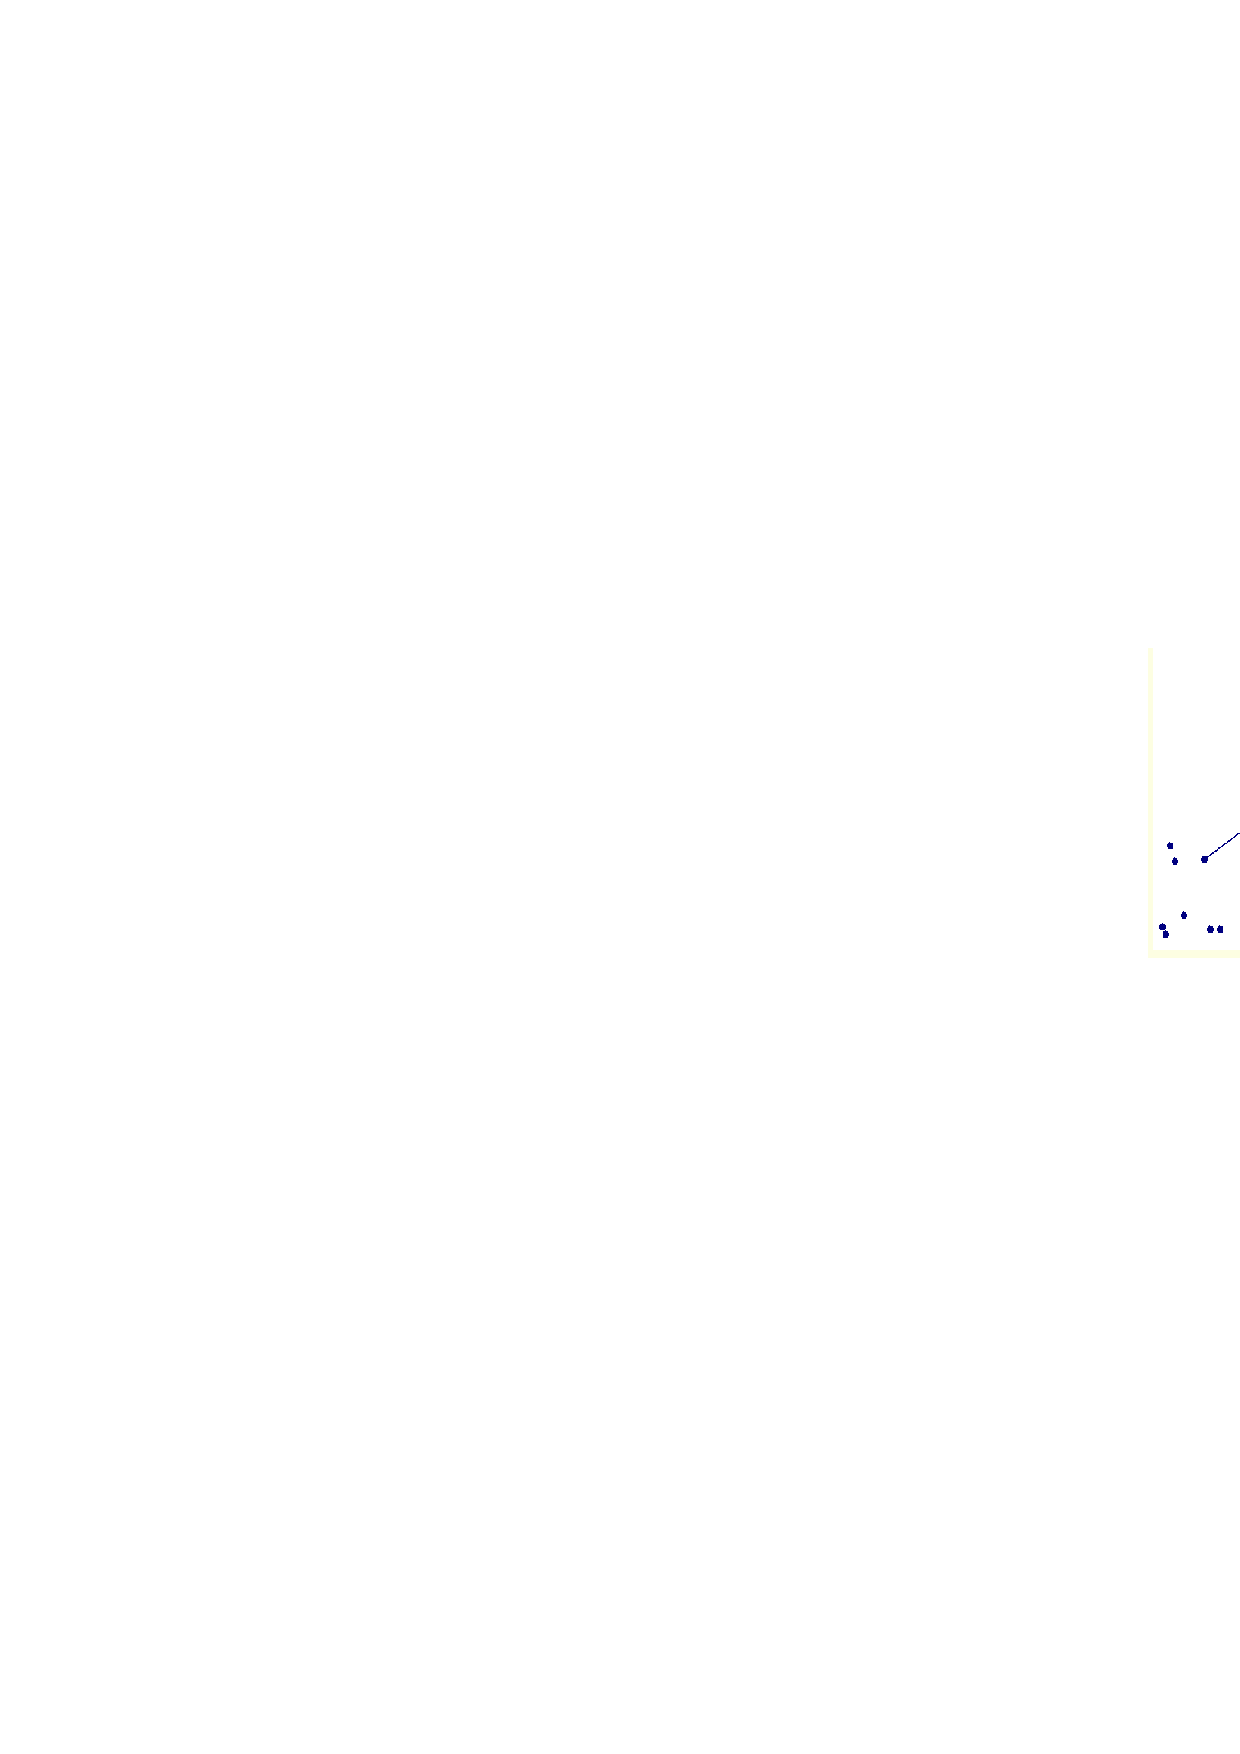
\includegraphics[width=2in]{single-linkage}
  
\end{slide}

\begin{slide}{Complete linkage}

\includegraphics[width=2.5in]{complete-linkage}

Also average linkage (obvious?)
  
\end{slide}

\begin{slide}{Ward's method example}

  \begin{itemize}
  \item Easiest to illustrate how Ward's method works by example.
  \item Data (one variable): 1, 2, 3, 7, 8, 9, 11, 12, 13. Suppose currently have 3 clusters 1,2,3; 7,8,9; 11,12,13. Measure dissimilarity by absolute difference (throw away minus sign).
  \item Which 2 of these 3 clusters to join together?
  \item Single-linkage distances: $7-3=4$, $11-3=8$, $11-9=2$; join 2nd and 3rd.
  \item Complete-linkage distances: $9-1=8$, $13-1=12$, $13-7=6$; also join 2nd and 3rd.
\end{itemize}
\end{slide}

\begin{slide}{\ldots continued}
\begin{itemize}
  \item Suppose join 1st 2 clusters. Joined cluster has mean $(1+2+3+7+8+9)/6=5$; new sum of squared distances from mean $(1-5)^2+(2-5)^2+(3-5)^2+(7-5)^2+(8-5)^2+(9-5)^2=58$.
  \item Join 1st and 3rd (obviously bad idea): mean now 7, sum of squared distances $(1-7)^2+(2-7)^2+(3-7)^2+(11-7)^2+(12-7)^2+(13-7)^2=154$.
  \item Join 2nd and 3rd: mean now 10, sum of squared distances $(7-10)^2+(8-10)^2+(9-10)^2+(11-10)^2+(12-10)^2+(13-10)^2=28$.
  \item Smallest of these three sums is 28, so join 2nd and 3rd clusters.
  \item Much computation, especially early with many clusters. But we don't care!
  \end{itemize}
  
\end{slide}

\begin{slide}{Ward's method in general}

  \begin{itemize}
  \item Work out sum of squared distances/dissimilarities from each observation to centre of its current cluster. Like error SS in ANOVA. Call it ESS.
  \item At start, each point in own cluster, so ESS 0.
  \item At each stage, join the two clusters that make resulting ESS smallest.
  \item Favours joining small clusters.
  \item Like linkage methods, joins ``similar'' clusters.
  \end{itemize}
  
\end{slide}

\begin{slide}{Dissimilarity data in SAS}

Dissimilarities for language data (first line for reference, not in data file):

{\scriptsize
\begin{verbatim}
  en no dk nl de fr es it pl hu sf
en 0  2  2  7  6  6  6  6  7  9  9
no 2  0  1  5  4  6  6  6  7  8  9
dk 2  1  0  6  5  6  5  5  6  8  9
nl 7  5  6  0  5  9  9  9 10  8  9
de 6  4  5  5  0  7  7  7  8  9  9
fr 6  6  6  9  7  0  2  1  5 10  9
es 6  6  5  9  7  2  0  1  3 10  9
it 6  6  5  9  7  1  1  0  4 10  8
pl 7  7  6 10  8  5  3  4  0 10  9
hu 9  8  8  8  9 10 10 10 10  0  8
sf 9  9  9  9  9  9  9  8  9  8  0
\end{verbatim}
}

SAS has special \verb-type=distance- for data like these:

\begin{verbatim}
data lang(type=distance);
	infile "one-ten.dat";
	input lang $ en no dk nl de fr es it pl hu sf;
\end{verbatim}

Variable \verb-lang- has names of languages; variable names given on \verb-input- line must match.

  
\end{slide}

\begin{slide}{Doing a hierarchical cluster analysis}

  \begin{itemize}
  \item Here, interested in clustering {\em process} more than final result, so hierarchical analysis appropriate: PROC CLUSTER.
  \item Choose single-linkage method for combining clusters (that is, combine clusters whose closest members are closest).
  \item Draw clustering ``tree'' from output data set. Trees by default vertical and (try to) use fancy graphics.

\begin{verbatim}
proc cluster method=single outtree=tree;
  id lang;

proc tree horizontal lineprinter;
  id lang;

\end{verbatim}
  \end{itemize}
  
\end{slide}

\begin{slide}{Output: cluster history}
  
{\scriptsize
\begin{verbatim}
                The CLUSTER Procedure
           Single Linkage Cluster Analysis

    Mean Distance Between Observations    6.672727


                   Cluster History
                                             Norm    T
                                              Min    i
  NCL    --Clusters Joined---      FREQ      Dist    e

   10    no          dk               2    0.1499    T
    9    fr          it               2    0.1499    T
    8    CL9         es               3    0.1499
    7    en          CL10             3    0.2997
    6    CL8         pl               4    0.4496
    5    CL7         de               4    0.5995
    4    CL5         nl               5    0.7493    T
    3    CL4         CL6              9    0.7493
    2    CL3         hu              10    1.1989    T
    1    CL2         sf              11    1.1989

\end{verbatim}
}

\end{slide}

\begin{slide}{Summary of clustering history}

  \begin{itemize}
  \item Join Norwegian and Danish.
  \item Join French and Italian.
  \item Join Spanish to the French-Italian cluster.
  \item Join English to the Norwegian-Danish cluster.
  \item Then: German and Dutch joined to Germanic languages cluster, Polish to Romance language cluster (!)
  \item Then join these two clusters together, and join Hungarian and Finnish to them.
  \end{itemize}

  
\end{slide}

\begin{slide}{Output from PROC TREE (read from {\em right})}

{\tiny
\begin{verbatim}
                            The TREE Procedure
                      Single Linkage Cluster Analysis

                        Minimum Distance Between Clusters

          1.2 1.1   1   0.9  0.8  0.7  0.6  0.5  0.4  0.3  0.2  0.1   0
          +----+----+----+----+----+----+----+----+----+----+----+----+
    N  en XXXXXXXXXXXXXXXXXXXXXXXXXXXXXXXXXXXXXXXXXXXXXX...............
    a     XXXXXXXXXXXXXXXXXXXXXXXXXXXXXXXXXXXXXXXXXXXXXX
    m  no XXXXXXXXXXXXXXXXXXXXXXXXXXXXXXXXXXXXXXXXXXXXXXXXXXXXXX.......
    e     XXXXXXXXXXXXXXXXXXXXXXXXXXXXXXXXXXXXXXXXXXXXXXXXXXXXXX
       dk XXXXXXXXXXXXXXXXXXXXXXXXXXXXXXXXXXXXXXXXXXXXXXXXXXXXXX.......
    o     XXXXXXXXXXXXXXXXXXXXXXXXXXXXXXX
    f  de XXXXXXXXXXXXXXXXXXXXXXXXXXXXXXX..............................
          XXXXXXXXXXXXXXXXXXXXXXXX
    O  nl XXXXXXXXXXXXXXXXXXXXXXXX.....................................
    b     XXXXXXXXXXXXXXXXXXXXXXXX
    s  fr XXXXXXXXXXXXXXXXXXXXXXXXXXXXXXXXXXXXXXXXXXXXXXXXXXXXXX.......
    e     XXXXXXXXXXXXXXXXXXXXXXXXXXXXXXXXXXXXXXXXXXXXXXXXXXXXXX
    r  it XXXXXXXXXXXXXXXXXXXXXXXXXXXXXXXXXXXXXXXXXXXXXXXXXXXXXX.......
    v     XXXXXXXXXXXXXXXXXXXXXXXXXXXXXXXXXXXXXXXXXXXXXXXXXXXXXX
    a  es XXXXXXXXXXXXXXXXXXXXXXXXXXXXXXXXXXXXXXXXXXXXXXXXXXXXXX.......
    t     XXXXXXXXXXXXXXXXXXXXXXXXXXXXXXXXXXXXXXX
    i  pl XXXXXXXXXXXXXXXXXXXXXXXXXXXXXXXXXXXXXXX......................
    o     X
    n  hu X............................................................
          X
       sf X............................................................

\end{verbatim}
}

\end{slide}

\begin{slide}{Checking our intuition about languages}

  \begin{itemize}
  \item Have a Germanic cluster (English, Norwegian, Danish, German, Dutch)
  \item Have a Romance cluster (French, Italian, Spanish, maybe Polish)
  \item Have two odd languages (Hungarian, Finnish).
  \item Corresponds to linguistics/geography pretty well (for such a crude measure).
  \item Maybe Dutch joins Germanic cluster late. Dutch number words much like German, but often happen not to start with same letter.
  \item Clustering method: single linkage may join languages that happen to have words starting with same letter, but not otherwise similar. Ward's method joins clusters that are more ``alike''. Change ``method='' on PROC DISCRIM line.
  \end{itemize}
  
\end{slide}

\begin{slide}{Tree from Ward's method}

{\tiny
\begin{verbatim}
                           The TREE Procedure
                 Ward's Minimum Variance Cluster Analysis

                             Semi-Partial R-Squared

        0.4   0.35     0.3    0.25     0.2    0.15     0.1    0.05      0
        +-------+-------+-------+-------+-------+-------+-------+-------+
     en        XXXXXXXXXXXXXXXXXXXXXXXXXXXXXXXXXXXXXXXXXXXXXXXXXXXXXXXX..
               XXXXXXXXXXXXXXXXXXXXXXXXXXXXXXXXXXXXXXXXXXXXXXXXXXXXXXXX
     no        XXXXXXXXXXXXXXXXXXXXXXXXXXXXXXXXXXXXXXXXXXXXXXXXXXXXXXXXXX
               XXXXXXXXXXXXXXXXXXXXXXXXXXXXXXXXXXXXXXXXXXXXXXXXXXXXXXXXXX
     dk        XXXXXXXXXXXXXXXXXXXXXXXXXXXXXXXXXXXXXXXXXXXXXXXXXXXXXXXXXX
               XXXXXXXXXXXXXXXXXXXXXXXXXXXXXXXXXXXXXXXX
     nl        XXXXXXXXXXXXXXXXXXXXXXXXXXXXXXXXXXXXXXXXXXXXXXXXXX........
               XXXXXXXXXXXXXXXXXXXXXXXXXXXXXXXXXXXXXXXXXXXXXXXXXX
  l  de        XXXXXXXXXXXXXXXXXXXXXXXXXXXXXXXXXXXXXXXXXXXXXXXXXX........
  a            XXXXXXXXXXXX
  n  hu        XXXXXXXXXXXXXXXXXXXXXXXXXXXXXXXXXXXXXX....................
  g            XXXXXXXXXXXXXXXXXXXXXXXXXXXXXXXXXXXXXX
     sf        XXXXXXXXXXXXXXXXXXXXXXXXXXXXXXXXXXXXXX....................
               X
     fr        XXXXXXXXXXXXXXXXXXXXXXXXXXXXXXXXXXXXXXXXXXXXXXXXXXXXXXXXXX
               XXXXXXXXXXXXXXXXXXXXXXXXXXXXXXXXXXXXXXXXXXXXXXXXXXXXXXXXXX
     it        XXXXXXXXXXXXXXXXXXXXXXXXXXXXXXXXXXXXXXXXXXXXXXXXXXXXXXXXXX
               XXXXXXXXXXXXXXXXXXXXXXXXXXXXXXXXXXXXXXXXXXXXXXXXXXXXXXXXX
     es        XXXXXXXXXXXXXXXXXXXXXXXXXXXXXXXXXXXXXXXXXXXXXXXXXXXXXXXXX.
               XXXXXXXXXXXXXXXXXXXXXXXXXXXXXXXXXXXXXXXXXXXXXXXXXX
     pl        XXXXXXXXXXXXXXXXXXXXXXXXXXXXXXXXXXXXXXXXXXXXXXXXXX........

\end{verbatim}
}
  
\end{slide}

\begin{slide}{Comparing single-linkage and Ward}

  \begin{itemize}
  \item In Ward, Dutch and German get joined earlier (before joining to Germanic cluster).
  \item Also Hungarian and Finnish get combined earlier.
  \item Consider which clustering method makes sense for data like these.
  \end{itemize}
  
\end{slide}

\begin{slide}{Another example}

Birth, death and infant mortality rates for 96 countries (variables not dissimilarities):

{\scriptsize
\begin{verbatim}
   24.7  5.7  30.8 Albania             12.5 11.9  14.4 Bulgaria
   13.4 11.7  11.3 Czechoslovakia      12   12.4   7.6 Former_E._Germany
   11.6 13.4  14.8 Hungary             14.3 10.2    16 Poland
   13.6 10.7  26.9 Romania               14    9  20.2 Yugoslavia
   17.7   10    23 USSR                15.2  9.5  13.1 Byelorussia_SSR
   13.4 11.6    13 Ukrainian_SSR       20.7  8.4  25.7 Argentina
   46.6   18   111 Bolivia             28.6  7.9    63 Brazil
   23.4  5.8  17.1 Chile               27.4  6.1    40 Columbia
   32.9  7.4    63 Ecuador             28.3  7.3    56 Guyana
...
\end{verbatim}
}

\begin{itemize}
\item Want to find groups of similar countries (and how many groups, which countries in each group).
\item Tree would be unwieldy with 96 countries.
\item More automatic way of finding number of clusters?
\item Two countries per line: how to read into SAS?
\end{itemize}
  
\end{slide}

\begin{slide}{SAS code and issues}

\begin{verbatim}
data birthrate;
  infile "birthrate.dat";
  input birth death infant country $ @@;

proc cluster method=average ccc standard;
  id country;
\end{verbatim}

\vspace{3ex}

  \begin{itemize}
  \item In DATA step, \verb=@@= means ``continue reading on same line''.
  \item Using average linkage.
  \item ``CCC'' is ``cubic clustering criterion'', helps us decide how many clusters.
  \item ``standard'' means to use standardized data (scaled to have mean 0 and SD 1) so each variable truly comparable.
  \end{itemize}

  
\end{slide}

\begin{slide}{Clustering history (a little)}

96 lines, just show some:

{\tiny
\begin{verbatim}
                                         Cluster History
                                                                                    Norm    T
                                                                                     RMS    i
       NCL    --Clusters Joined---      FREQ     SPRSQ     RSQ    ERSQ     CCC      Dist    e

        96    Austria     Canada           2    0.0000    1.00    .        .      0.0165
        95    Czechosl    Ukrainia         2    0.0000    1.00    .        .      0.0175 
...
        20    CL82        CL34             6    0.0016    .967    .        .      0.2664
        19    CL32        CL38             7    0.0018    .965    .952    4.10    0.2709
        18    Bolivia     CL29             6    0.0011    .964    .949    4.53    0.2794
        17    CL21        Oman             6    0.0014    .963    .945    4.87    0.3191
        16    CL23        CL26            16    0.0059    .957    .942    3.84    0.3225 
...
         8    CL12        CL74            24    0.0067    .907    .887    2.16    0.4773
         7    Mexico      Korea            2    0.0026    .904    .873    3.27    0.5037
         6    Afghanis    CL13             8    0.0045    .900    .854    4.47    0.5328
         5    CL15        CL10            45    0.0517    .848    .827    1.57    0.5697
         4    CL9         CL8             42    0.1001    .748    .788    -2.3    0.7742
         3    CL5         CL4             87    0.3980    .350    .723     -12    1.0708
         2    CL3         CL7             89    0.0385    .311    .593    -6.8    1.1662
         1    CL2         CL6             97    0.3114    .000    .000    0.00    1.5693

\end{verbatim}
}

Look for large values of CCC compared to neighbours, here 17 clusters or 6. We'll try 6.
  
\end{slide}

\begin{slide}{The 6 best clusters}

  \begin{itemize}
  \item Only purpose for running previous analysis was to get good number of clusters.
  \item 6 clusters obtained by ``chopping the tree'' may not be best division of countries into 6 clusters.
  \item Do better by deciding on 6 (or however many) clusters first, {\em then} trying for best division of countries into 6 clusters.
  \item This is where K-means clustering comes in. Choose best division of individuals (countries) into K (6) clusters so that sum of squared distances from individuals to cluster averages made smallest (over all possible divisions into K clusters).
  \item Use PROC FASTCLUS (which does not have ``standard'' option so have to standardize first).
\end{itemize}

\end{slide}

\begin{slide}{Code}

\begin{verbatim}
proc standard mean=0 std=1;

proc fastclus maxclusters=6 out=clust;
  id country;

proc sort data=clust;
  by cluster;

proc print data=clust;
  by cluster;
\end{verbatim}

Sort data by cluster and print sorted data.
  
\end{slide}

\begin{slide}{Cluster means and SDs}

{\scriptsize
\begin{verbatim}
                          Cluster Means

  Cluster             birth             death            infant
  =============================================================
     1         -0.435769031      -1.143859869      -0.728110805
     2          1.204946595       0.697233337       1.016509747
     3          1.301924159       2.117634622       1.866220472
     4         -0.219972241       2.111657686      -0.454443499
     5         -1.173710389      -0.185637473      -0.953436985
     6          0.416099253      -0.516998811       0.264875362

                   Cluster Standard Deviations

  Cluster             birth             death            infant
  =============================================================
     1         0.3560992452      0.3384785179      0.2086886380
     2         0.2838078359      0.3886873578      0.4595354494
     3         0.2072519523      0.4982442191      0.4178547653
     4         0.2870875322      0.7759545638      0.2767385711
     5         0.1523496837      0.3449633244      0.1225870222
     6         0.3884813426      0.2398267650      0.4102515861
\end{verbatim}
}


\end{slide}

\begin{slide}{Cluster membership}

{\scriptsize
\begin{verbatim}
--------------------------- Cluster=1 --------------------------------------------

 Obs      birth       death      infant     country     DISTANCE

   1    -0.33439    -1.10513    -0.52402    Albania      0.17862
   2    -0.62967    -0.52417    -0.63491    Argentin     0.53740
   3    -0.43036    -1.08361    -0.82189    Chile        0.18142
   4    -0.13508    -1.01906    -0.32399    Columbia     0.42671
   5    -0.12770    -1.38485    -0.68709    Venezuel     0.46416
   6    -0.06126    -1.51395    -0.84581    Bahrain      0.63514
   7    -0.51156    -0.97603    -0.98279    Israel       0.34370
   8    -0.17937    -1.85822    -0.85451    Kuwait       0.89881
   9    -0.47465    -1.51395    -0.62838    United_A     0.51244
  10    -0.59276    -0.88996    -0.49793    China        0.27987
  11    -1.29403    -1.27727    -1.06106    Hong_Kon     1.01806
  12     0.17496    -1.12665    -0.67187    Malaysia     0.58493
  13    -0.84374    -1.21271    -1.03062    Singapor     0.61480
  14    -0.58538    -0.99754    -0.77189    Sri_Lank     0.21867
  15    -0.51156    -0.67479    -0.58490    Thailand     0.36033
\end{verbatim}
}

\end{slide}

\begin{slide}{Cluster 2}

{\scriptsize
\begin{verbatim}
--------------------------- Cluster=2 --------------------------------------------

   Obs     birth      death      infant    country     DISTANCE

    16    0.97958    0.14285    1.15669    Iran         0.53619
    17    0.95744    1.00353    1.39368    Banglade     0.73436
    18    0.89838    1.24022    1.63285    Cambodia     1.07380
    19    0.76551    0.85291    1.58936    Nepal        0.88866
    20    1.42249    0.16437    0.26306    Botswana     0.75211
    21    1.24533    0.80988    0.39352    Congo        0.53986
    22    0.75074    1.28325    1.04580    Gabon        0.86684
    23    1.11984    0.48713    0.76314    Ghana        0.12230
    24    1.31177    0.09982    0.37178    Kenya        0.67632
    25    1.09031    0.27196    1.74156    Namibia      0.92807
    26    1.42249    1.02505    1.08928    Nigeria      0.58894
    27    1.13460    1.06808    1.15451    Sudan        0.60039
    28    1.29700    0.35802    1.37194    Swazilan     0.56207
    29    1.69562    1.02505    1.04580    Uganda       0.73647
    30    1.57013    0.68078    1.11103    Tanzania     0.49353
    31    1.20842    0.72381    0.61095    Zaire        0.30705
    32    1.61442    0.61623    0.54572    Zambia       0.54965

\end{verbatim}
}

  
\end{slide}

\begin{slide}{Cluster 3 and 4}

{\scriptsize
\begin{verbatim}
--------------------------- Cluster=3 --------------------------------------------

   Obs     birth      death      infant    country     DISTANCE

    33    1.28224    1.54146    1.21974    Bolivia      0.97448
    34    0.82456    1.69208    2.75477    Afghanis     1.06314
    35    1.32653    2.01483    1.78505    Angola       0.23936
    36    1.42988    2.12242    1.78505    Ethiopia     0.21566
    37    1.34129    2.27303    1.91550    Gambia       0.09648
    38    1.40773    3.04765    1.63285    Malawi       0.91953
    39    1.16413    1.64904    1.87202    Mozambiq     0.56353
    40    1.40035    2.70337    2.15467    Sierra_L     0.56234
    41    1.54060    2.01483    1.67633    Somalia      0.39955


--------------------------- Cluster=4 --------------------------------------------

  Obs      birth      death      infant     country    DISTANCE

   42    -0.01697    2.66034    -0.25876    Mexico      0.61689
   43    -0.42297    1.56297    -0.65013    Korea       0.61689


\end{verbatim}
}
  
\end{slide}

\begin{slide}{Cluster 5}

{\tiny
\begin{verbatim}
  Obs      birth       death      infant     country     DISTANCE
   44    -1.23498     0.22892    -0.88060    Bulgaria     0.33826
   45    -1.16854     0.18589    -0.94800    Czechosl     0.28590
   46    -1.27189     0.33651    -1.02845    Former_E     0.45403
   47    -1.30142     0.55168    -0.87190    Hungary      0.66583
   48    -1.10211    -0.13687    -0.84581    Poland       0.12899
   49    -1.15378    -0.02928    -0.60882    Romania      0.34023
   50    -1.12425    -0.39507    -0.75449    Yugoslav     0.35379
   51    -0.85112    -0.17990    -0.69361    USSR         0.42007
   52    -1.03567    -0.28748    -0.90886    Byelorus     0.23981
   53    -1.16854     0.16437    -0.91104    Ukrainia     0.26595
   54    -0.82898    -0.26597    -0.71753    Uruguay      0.44895
   55    -1.27189    -0.05080    -1.02193    Belgium      0.13118
   56    -1.18331    -0.15838    -1.06759    Finland      0.13997
   57    -1.24236     0.22892    -1.03062    Denmark      0.34609
   58    -1.15378    -0.30900    -1.03280    France       0.23045
   59    -1.31618     0.07830    -1.03280    Germany      0.24157
   60    -1.41214    -0.35204    -0.95452    Greece       0.34233
   61    -1.04305    -0.37355    -1.03062    Ireland      0.31979
   62    -1.44167    -0.37355    -1.00236    Italy        0.38293
   63    -1.18331    -0.48114    -1.03932    Netherla     0.39409
   64    -1.10211    -0.02928    -1.02410    Norway       0.13492
   65    -1.27927    -0.28748    -0.90886    Portugal     0.21422
   66    -1.36785    -0.56721    -1.01758    Spain        0.50927
   67    -1.08734     0.05679    -1.07193    Sweden       0.22485
   68    -1.23498    -0.28748    -1.03932    Switzerl     0.21892
   69    -1.15378     0.14285    -1.01105    U.K.         0.25402
   70    -1.05781    -0.73934    -1.01975    Austria      0.65632
   71    -1.42691    -0.88996    -1.09585    Japan        0.84206
   72    -1.08734    -0.76086    -1.03715    Canada       0.67483
   73    -0.92494    -0.58872    -0.99584    U.S.A.       0.55498

\end{verbatim}
}
  
\end{slide}

\begin{slide}{Cluster 6}

{\tiny
\begin{verbatim}
  Obs      birth       death      infant     country     DISTANCE
   74    -0.04650    -0.63176     0.17609    Brazil       0.47528
   75     0.27092    -0.73934     0.17609    Ecuador      0.38853
   76    -0.06864    -0.76086     0.02389    Guyana       0.63871
   77     0.41118    -0.91148    -0.28050    Paraguay     0.86208
   78     0.27092    -0.54569     1.19582    Peru         0.75143
   79     0.98696    -0.65327     0.30655    Iraq         0.72179
   80     0.71383    -0.95451    -0.23702    Jordan       0.93690
   81     0.18234    -0.45962    -0.15005    Lebanon      0.61194
   82     1.20842    -0.65327    -0.32399    Oman         1.20413
   83     0.95005    -0.69631     0.35003    Saudi_Ar     0.69244
   84    -0.00221    -0.52417     0.45875    Turkey       0.31280
   85     0.09376    -0.13687     0.78489    India        0.51477
   86    -0.04650    -0.30900     0.43700    Indonesi     0.38480
   87     0.50714    -0.43810     0.28481    Mongolia     0.26224
   88     0.07899    -0.58872     1.14799    Pakistan     0.74443
   89     0.29307    -0.67479    -0.21527    Philippi     0.69706
   90     0.18972    -0.28748     0.19784    Vietnam      0.32897
   91     0.46285    -0.54569     0.41526    Algeria      0.18049
   92     0.70645    -0.28748    -0.11961    Egypt        0.71885
   93     1.09031    -0.30900     0.58920    Libya        0.81294
   94     0.46285    -0.22293     0.58920    Morocco      0.32133
   95     0.21187    -0.20142     0.37178    South_Af     0.29044
   96     0.13805    -0.76086    -0.06308    Tunisia      0.61470
   97     0.92053    -0.11535     0.24132    Zimbabwe     0.73814

\end{verbatim}
}
  
\end{slide}

\begin{slide}{Summary of clusters}

  \begin{itemize}
  \item Cluster 3 has highest means on all variables; describe as ``very poor'' countries.
  \item Cluster 2 also higher than average on all, but not as high as Cluster 3:''poor'' but not ``very poor''.
  \item Cluster 4 has high death rate but low birth rates and infant mortality rates: ``would-be western''.
  \item Cluster 6 has slightly above-average birth and infant mortality rates, and lower-than-average death rate: ``third world''.
  \item Cluster 1 has lower-than-average everything, and especially low death rate: ``becoming western''.
  \item Cluster 5 also is low on everything, and especially low on birth rate: ``western world''.
  \item New variable ``distance'' shows how far a country is from its cluster average. Small value means ``typical of its cluster''; large implies ``does not fit any cluster very well''. Eg.\ Afghanistan vs.\ cluster 3.
  \end{itemize}
  
\end{slide}

\begin{slide}{Using PROC DISCRIM on clusters}

  \begin{itemize}
  \item Summary on previous page took some working out.
  \item Idea: use output clusters as ``grouping'' variable for PROC DISCRIM with ``can'' option: get canonical variables that might shed some light on how clusters differ.
  \item Code below. Add onto end of previous (uses output data set with cluster membership in it):
\begin{verbatim}
proc discrim can out=zz;
  class cluster;
  var birth death infant;

proc sort;
  by cluster;

proc print;
  var country birth death infant can1 can2 can3;
  by cluster;

\end{verbatim}
  \end{itemize}
  
\end{slide}

\begin{slide}{Output from discriminant analysis}

{\scriptsize
\begin{verbatim}
                           The DISCRIM Procedure

         Observations      97          DF Total                96
         Variables          3          DF Within Classes       91
         Classes            6          DF Between Classes       5

                                Eigenvalues of Inv(E)*H
                                  = CanRsq/(1-CanRsq)
                  Eigenvalue    Difference    Proportion    Cumulative

            1       25.2031       20.7304        0.8449        0.8449
            2        4.4727        4.3181        0.1499        0.9948
            3        0.1546                      0.0052        1.0000

               Test of H0: The canonical correlations in the
                  current row and all that follow are zero
                Likelihood    Approximate
                     Ratio        F Value    Num DF    Den DF    Pr > F

           1    0.00603979          88.02        15    246.09    <.0001
           2    0.15826107          34.06         8       180    <.0001
           3    0.86611339           4.69         3        91    0.0043

\end{verbatim}
}


\end{slide}

\begin{slide}{The canonical variables}

3 canonical variables possible, all significant (though eigenvalue for last very small).
  
{\scriptsize
\begin{verbatim}
                       Raw Canonical Coefficients
      Variable              Can1              Can2              Can3
      birth          2.706578482      -1.095888137      -1.935532844
      death          0.683696755       2.777557832      -0.585485143
      infant         2.017039026      -0.834166707       2.334460951
\end{verbatim}
}

\begin{itemize}
\item Can1 positive where birth rate and infant mortality rate both high, negative where both low.
\item Can2 positive where death rate high, negative where low.
\item Can3 positive where infant mortality rate high compared to birth rate, negative where low.
\end{itemize}
  
\end{slide}

\begin{slide}{The clusters}

{\scriptsize
\begin{verbatim}

                     Class Means on Canonical Variables
       CLUSTER              Can1              Can2              Can3
             1      -3.430124271      -2.092217034      -0.186588012
             2       5.788318527      -0.231819353      -0.367431160
             3       8.735819354       2.898350402       0.596858239
             4      -0.068268900       6.485397951      -1.871461306
             5      -5.226778630       1.565961865       0.154681580
             6       1.306998818      -2.112942540       0.115662540


\end{verbatim}
}

\begin{enumerate}
\item Low on everything (Chile).
\item High birth and infant mortality, average death rate (Ghana).
\item High (or very high) on everything (Gambia).
\item High death rate, high birth rate compared to infant mortality rate (Mexico).
\item Very low birth and infant mortality, highish death rate (Canada).
\item High birth and infant mortality but low death rate (Algeria).
\end{enumerate}
  
\end{slide}

\begin{slide}{Final example: a hockey league}

  \begin{itemize}
  \item 
An Ontario hockey league has teams in 21 cities. How can we arrange those teams into 4 geographical divisions?
\item Distance data in spreadsheet.
\item Take out spaces in team names.
\item Save as ``text/csv'', and use text editor to remove all double-quotes.
\item Open new file on Mathlab.
\item Copy lines with team names and distances to clipboard, paste into Mathlab file.
\item PROC FASTCLUS doesn't work on distance data, so go back to PROC CLUSTER.

  \end{itemize}
  
\end{slide}

\begin{slide}{A map}
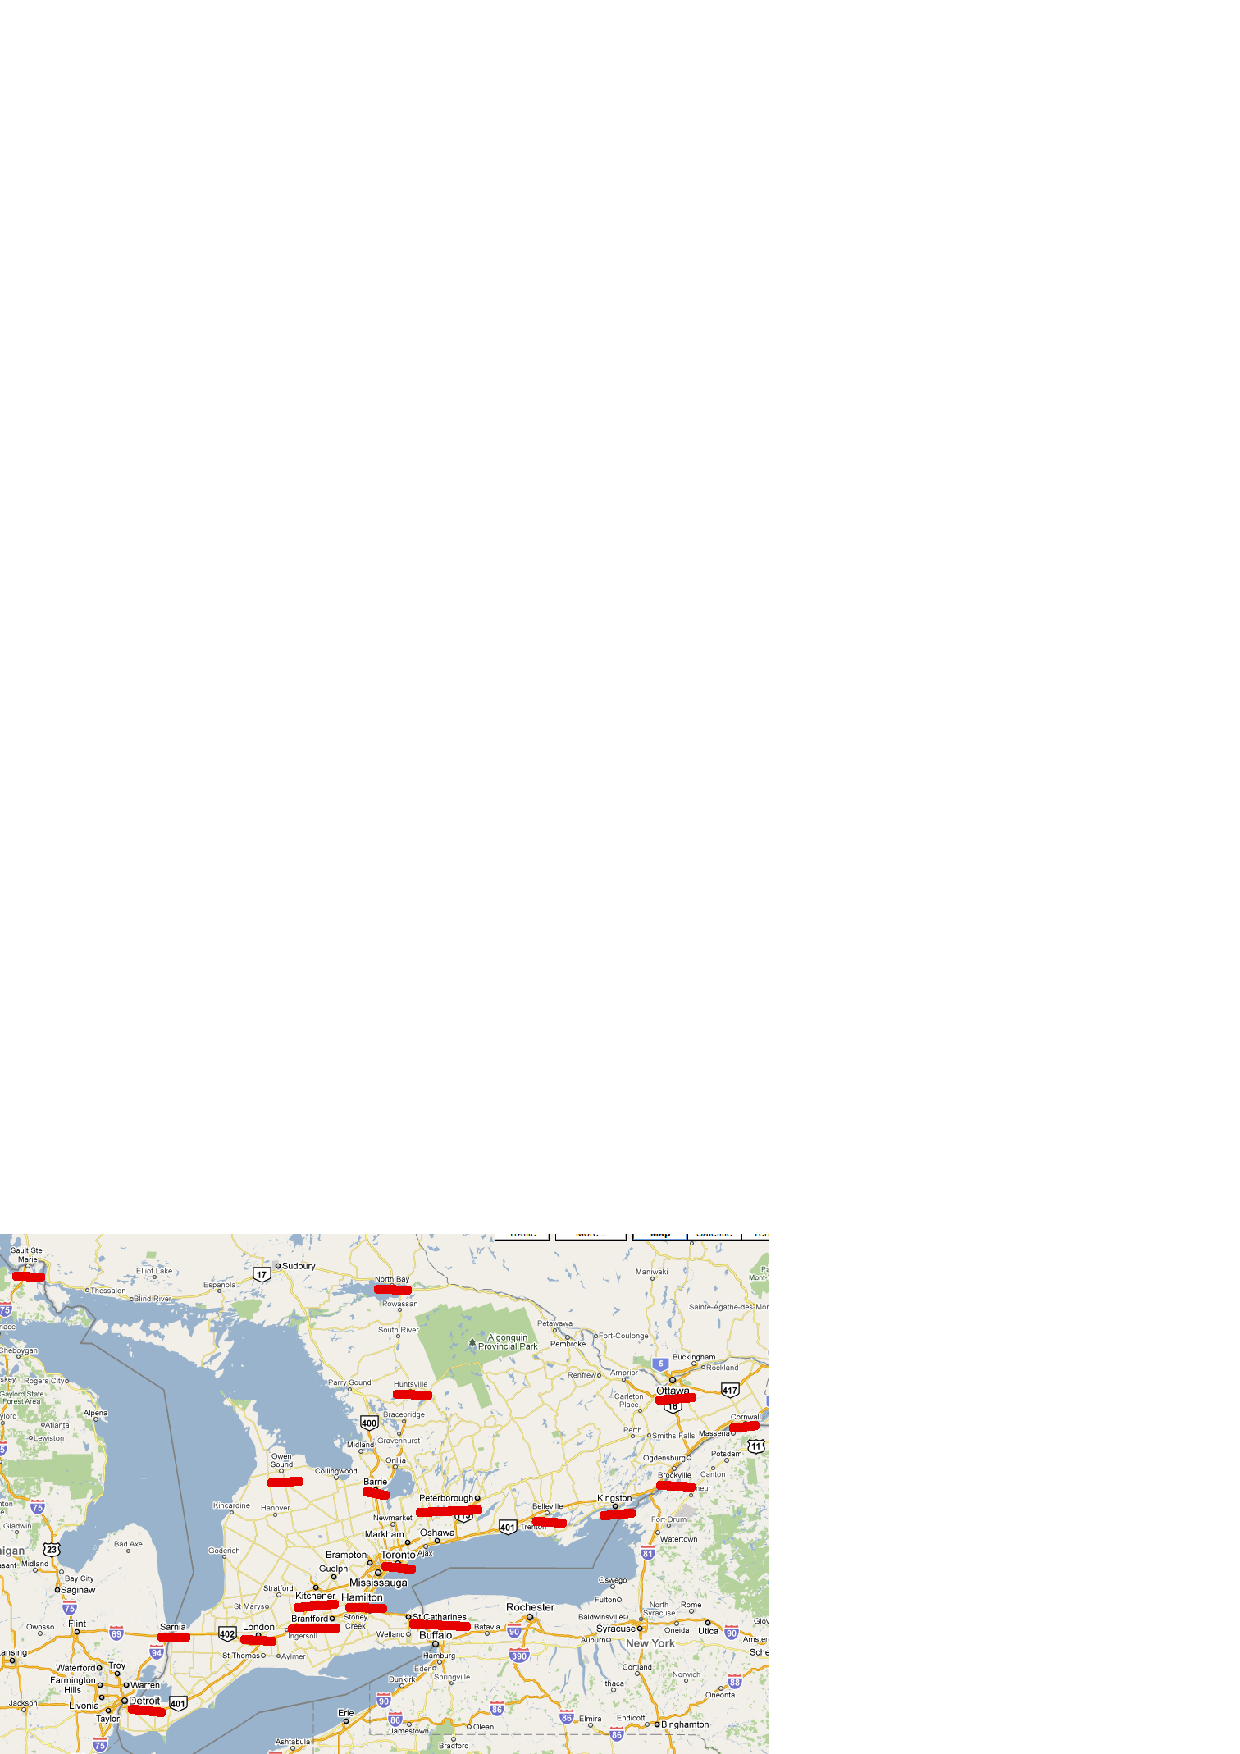
\includegraphics[width=4.5in]{ontario2}
  \end{slide}

\begin{slide}{My code}

\begin{verbatim}
options linesize=75;

data dist(type=distance);
  infile "ontario-road-distances.dat" delimiter=",";
  input team $ Barrie Belleville Brantford Brockville 
    Cornwall Hamilton Huntsville Kingston Kitchener 
    London NiagaraFalls NorthBay Ottawa OwenSound 
    Peterborough Sarnia SaultSteMarie StCatharines 
    ThunderBay Toronto Windsor;

proc cluster method=ward outtree=tree;
  id team;

proc tree horizontal lineprinter;
  id team;
\end{verbatim}

Use same team names in same order as data file. Hope tree output gives some idea of which teams to place in which divisions.
  
\end{slide}

\begin{slide}{Clustering history}

{\scriptsize
\begin{verbatim}
                              Cluster History           Norm    T
                                                         RMS    i
             NCL    --Clusters Joined---      FREQ      Dist    e
              20    NiagaraF    StCathar         2    0.0339     
              19    Brantfor    Hamilton         2    0.0678    T
              18    CL19        Kitchene         3    0.0864     
              17    Bellevil    Kingston         2    0.1271     
              16    CL18        Toronto          4    0.1489     
              15    Brockvil    Cornwall         2     0.161     
              14    London      Sarnia           2    0.1695     
              13    CL16        CL20             6    0.1742     
              12    CL15        Ottawa           3    0.1782     
              11    Barrie      OwenSoun         2    0.2034     
              10    Huntsvil    NorthBay         2    0.2203     
               9    CL17        Peterbor         3    0.2497     
               8    CL14        Windsor          3    0.2977     
               7    CL11        CL13             8    0.3246     
               6    CL9         CL12             6    0.3842     
               5    CL7         CL8             11    0.4606     
               4    CL6         CL10             8    0.6431     
               3    CL5         CL4             19    0.7445     
               2    SaultSte    ThunderB         2    1.1694     
               1    CL3         CL2             21    1.9625     

\end{verbatim}
}
  
\end{slide}


\begin{slide}{The tree}

{\tiny
\begin{verbatim}
                          Average Distance Between Clusters

             2    1.8   1.6   1.4   1.2    1    0.8   0.6   0.4   0.2    0
             +-----+-----+-----+-----+-----+-----+-----+-----+-----+-----+
      Barrie  XXXXXXXXXXXXXXXXXXXXXXXXXXXXXXXXXXXXXXXXXXXXXXXXXXXXXX......
              XXXXXXXXXXXXXXXXXXXXXXXXXXXXXXXXXXXXXXXXXXXXXXXXXXXXXX
    OwenSoun  XXXXXXXXXXXXXXXXXXXXXXXXXXXXXXXXXXXXXXXXXXXXXXXXXXXXXX......
              XXXXXXXXXXXXXXXXXXXXXXXXXXXXXXXXXXXXXXXXXXXXXXXXXX
    Brantfor  XXXXXXXXXXXXXXXXXXXXXXXXXXXXXXXXXXXXXXXXXXXXXXXXXXXXXXXXXX..
              XXXXXXXXXXXXXXXXXXXXXXXXXXXXXXXXXXXXXXXXXXXXXXXXXXXXXXXXXX
    Hamilton  XXXXXXXXXXXXXXXXXXXXXXXXXXXXXXXXXXXXXXXXXXXXXXXXXXXXXXXXXX..
              XXXXXXXXXXXXXXXXXXXXXXXXXXXXXXXXXXXXXXXXXXXXXXXXXXXXXXXXX
    Kitchene  XXXXXXXXXXXXXXXXXXXXXXXXXXXXXXXXXXXXXXXXXXXXXXXXXXXXXXXXX...
              XXXXXXXXXXXXXXXXXXXXXXXXXXXXXXXXXXXXXXXXXXXXXXXXXXXXXXXX
     Toronto  XXXXXXXXXXXXXXXXXXXXXXXXXXXXXXXXXXXXXXXXXXXXXXXXXXXXXXXX....
              XXXXXXXXXXXXXXXXXXXXXXXXXXXXXXXXXXXXXXXXXXXXXXXXXXXXXXX
    NiagaraF  XXXXXXXXXXXXXXXXXXXXXXXXXXXXXXXXXXXXXXXXXXXXXXXXXXXXXXXXXXX.
              XXXXXXXXXXXXXXXXXXXXXXXXXXXXXXXXXXXXXXXXXXXXXXXXXXXXXXXXXXX
    StCathar  XXXXXXXXXXXXXXXXXXXXXXXXXXXXXXXXXXXXXXXXXXXXXXXXXXXXXXXXXXX.
              XXXXXXXXXXXXXXXXXXXXXXXXXXXXXXXXXXXXXXXXXXXXXX
      London  XXXXXXXXXXXXXXXXXXXXXXXXXXXXXXXXXXXXXXXXXXXXXXXXXXXXXXX.....
              XXXXXXXXXXXXXXXXXXXXXXXXXXXXXXXXXXXXXXXXXXXXXXXXXXXXXXX
 t    Sarnia  XXXXXXXXXXXXXXXXXXXXXXXXXXXXXXXXXXXXXXXXXXXXXXXXXXXXXXX.....
 e            XXXXXXXXXXXXXXXXXXXXXXXXXXXXXXXXXXXXXXXXXXXXXXXXXXX
 a   Windsor  XXXXXXXXXXXXXXXXXXXXXXXXXXXXXXXXXXXXXXXXXXXXXXXXXXX.........
 m            XXXXXXXXXXXXXXXXXXXXXXXXXXXXXXXXXXXXXX
\end{verbatim}
}
\end{slide}

\begin{slide}{The rest}
{\tiny
\begin{verbatim}
              2    1.8   1.6   1.4   1.2    1    0.8   0.6   0.4   0.2    0
              +-----+-----+-----+-----+-----+-----+-----+-----+-----+-----+
    Bellevil  XXXXXXXXXXXXXXXXXXXXXXXXXXXXXXXXXXXXXXXXXXXXXXXXXXXXXXXX....
              XXXXXXXXXXXXXXXXXXXXXXXXXXXXXXXXXXXXXXXXXXXXXXXXXXXXXXXX
    Kingston  XXXXXXXXXXXXXXXXXXXXXXXXXXXXXXXXXXXXXXXXXXXXXXXXXXXXXXXX....
              XXXXXXXXXXXXXXXXXXXXXXXXXXXXXXXXXXXXXXXXXXXXXXXXXXXXX
    Peterbor  XXXXXXXXXXXXXXXXXXXXXXXXXXXXXXXXXXXXXXXXXXXXXXXXXXXXX.......
              XXXXXXXXXXXXXXXXXXXXXXXXXXXXXXXXXXXXXXXXXXXXXXXX
    Brockvil  XXXXXXXXXXXXXXXXXXXXXXXXXXXXXXXXXXXXXXXXXXXXXXXXXXXXXXX.....
              XXXXXXXXXXXXXXXXXXXXXXXXXXXXXXXXXXXXXXXXXXXXXXXXXXXXXXX
    Cornwall  XXXXXXXXXXXXXXXXXXXXXXXXXXXXXXXXXXXXXXXXXXXXXXXXXXXXXXX.....
              XXXXXXXXXXXXXXXXXXXXXXXXXXXXXXXXXXXXXXXXXXXXXXXXXXXXXXX
      Ottawa  XXXXXXXXXXXXXXXXXXXXXXXXXXXXXXXXXXXXXXXXXXXXXXXXXXXXXXX.....
              XXXXXXXXXXXXXXXXXXXXXXXXXXXXXXXXXXXXXXXXX
    Huntsvil  XXXXXXXXXXXXXXXXXXXXXXXXXXXXXXXXXXXXXXXXXXXXXXXXXXXXX.......
              XXXXXXXXXXXXXXXXXXXXXXXXXXXXXXXXXXXXXXXXXXXXXXXXXXXXX
    NorthBay  XXXXXXXXXXXXXXXXXXXXXXXXXXXXXXXXXXXXXXXXXXXXXXXXXXXXX.......
              X
    SaultSte  XXXXXXXXXXXXXXXXXXXXXXXXX...................................
              XXXXXXXXXXXXXXXXXXXXXXXXX
    ThunderB  XXXXXXXXXXXXXXXXXXXXXXXXX...................................

\end{verbatim}
}
  
\end{slide}

\begin{slide}{Splitting into divisions, 1st try}

  \begin{itemize}
  \item Sault Ste Marie and Thunder Bay are very distant from everywhere else.
  \item Clustering history says 4 clusters between distance 0.6431 and 0.7445, so ``chop tree'' there, to get:
    \begin{itemize}
    \item Sault Ste Marie
    \item Thunder Bay
    \item Belleville, Kingston, Peterborough, Brockville, Cornwall, Ottawa, Huntsville, North Bay (8 teams)
    \item the rest (11 teams)
    \end{itemize}
\item Divisions of 1 team make no sense, so try splitting big divisions  and placing 2 northernmost teams somewhere.
  \end{itemize}
  
\end{slide}

\begin{slide}{2nd try}

  \begin{itemize}
  \item Next split at distance 0.6431 splits Huntsville and North Bay from the eastern teams. Place them in a northern division with Sault Ste Marie and Thunder Bay.
  \item Next split at distance 0.4606 splits London, Sarnia and Windsor off from the big group. That leaves us with this:
    \begin{itemize}
    \item (north, 4) Huntsville, North Bay, Sault Ste Marie, Thunder Bay
    \item (east, 6) Belleville, Kingston, Peterborough, Brockville, Cornwall, Ottawa
    \item (west, 3) London, Sarnia, Windsor
    \item (south, 8) Niagara Falls, St Catharines, Brantford, Hamilton, Kitchener, Toronto, Barrie, Owen Sound
    \end{itemize}
  \item That's not too bad. Getting the divisions to be the same size is beyond our scope!
  \end{itemize}
  
\end{slide}

\begin{slide}{Another map}

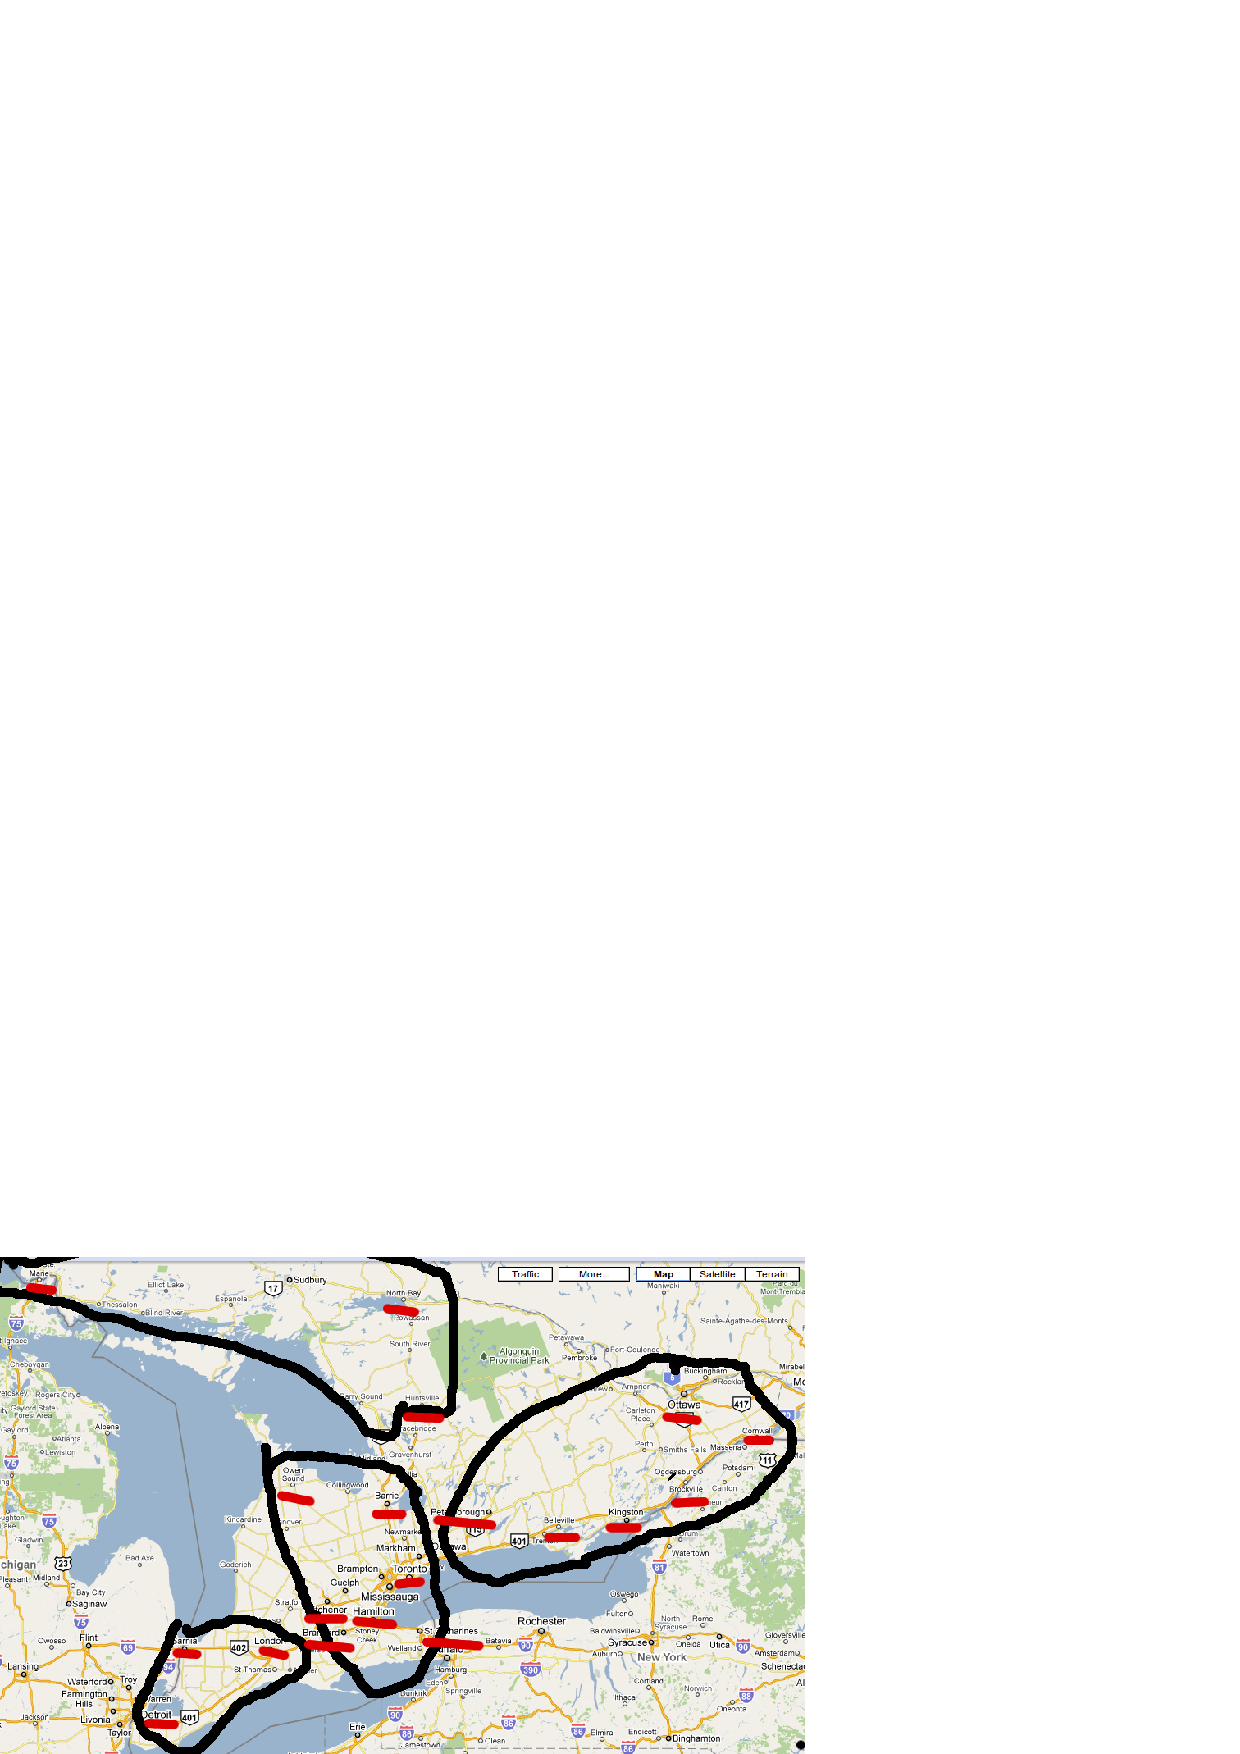
\includegraphics[width=4.5in]{ontario}
  
\end{slide}

\end{document}
